%!TEX root = ./ERL Industrial Robots-nutshell.tex

%++++++++++++++++++++++++++++++++++++++++++++++++++++++++++++++++++++
%--------------------------------------------------------------------
%++++++++++++++++++++++++++++++++++++++++++++++++++++++++++++++++++++
\phantomsection
\section{Introduction}
\label{sec:nutshell-introduction}

The objective of the \erl is to organize several indoor robot competition events per year, ensuring a
scientific competition format, around the following two challenges: \erlsrlong and \erlirlong.\\
Those indoor robot competitions will be focused on two major challenges addressed by H2020: societal
challenges (service robots helping and interacting with humans at home, especially the elderly and
those with motor disabilities) and industrial leadership (industrial robots addressing the flexible factories of the future and modern automation issues). These challenges were addressed by \roah and \roaw and will be extended in the \erl by building on the current version of the
rule books and testbeds designed and used during RoCKIn’s project lifetime.\\
Thereby, the \erl competitions pave the way for technology transfer and contribute to the continued commercial competitiveness of European industry. 

%--------------------------------------------------------------------
%--------------------------------------------------------------------
%--------------------------------------------------------------------
\clearpage
\phantomsection
\section{The \erlir User Story}

The \erlir competition considers a medium-sized factory \rollin trying to optimize its production process to meet the increasing demands of their customers. 
\rollin is specialized in production of small- to medium-sized lots of mechanical parts and assembled mechatronic products. 
Furthermore, the \rollin production line integrates incoming shipments of damaged or unwanted products and raw material. 
\rollin's operation is quite dynamic; each costumer order is unique. 

In today's production lines customization grows more and more. 
This results in smaller lot sizes, more individual and more flexible production processes. 
Nevertheless automation is necessary to guarantee a reliable and a cost efficient production.
Therefore, \rollin plans to utilize mobile robots to assist workers in complex  tasks such as assembly processes, quality controls, order handling and logistics. 
The robots have to be able to switch between different tasks autonomously. They operate machines (for drilling, milling as well as assembling), transport items and assist workers in manual operations. 
This connection of human workers and mobile robot assistants optimizes the whole production by combining human versatility and robotic accuracy and reliability.

The \erlir competition is looking for ways towards innovative and flexible manufacturing systems such as required by the \rollin factory. The challenges for such a system are set in the subsequent scenario description.


%--------------------------------------------------------------------
%--------------------------------------------------------------------
%--------------------------------------------------------------------
\clearpage
\phantomsection
\section{\erlir Scenario}

The \erlir scenario description is structured into three parts: environment, tasks, and robots. Those constitute the first part of the rules for the competition:
%
\begin{itemize}
\item The environment part specifies the environment in which the tasks have to be performed. This information is relevant for building testbeds and simulators.
\item The tasks part provides information on the tasks that the participating teams are expected to solve through the use of one or more robots and possibly additional equipment. 
This information tells the participating teams what to prepare for.
\item The robot part specifies some constraints and requirements for participating robots, which mainly arise for practical reasons (size and weight limitations, for example) and/or due to the need to observe safety regulations.
\end{itemize}

%--------------------------------------------------------------------
%--------------------------------------------------------------------
\subsection{\erlir Environment}

The \erlir environment uses a scaled-down environment typical for a small- to medium-sized factory production area, including all its environmental aspects like walls, workstation areas, shelves, machinery and supply devices like conveyor belts. 
Figure \ref{fig:rockin-n-rollin-production-area-nutshell} shows the evolution of the \erlir environment from its early concept in \roaw to its implementation in the second \roaw competition in Lisbon in November 2015. More detailed specifications are given in the rule book of \erlir.\\

%
\begin{figure}[htb]
  \begin{center}
  	\hfill
	  \subfigure[Early concept]{
		  \scalebox{1.0}[1.0]{
  		  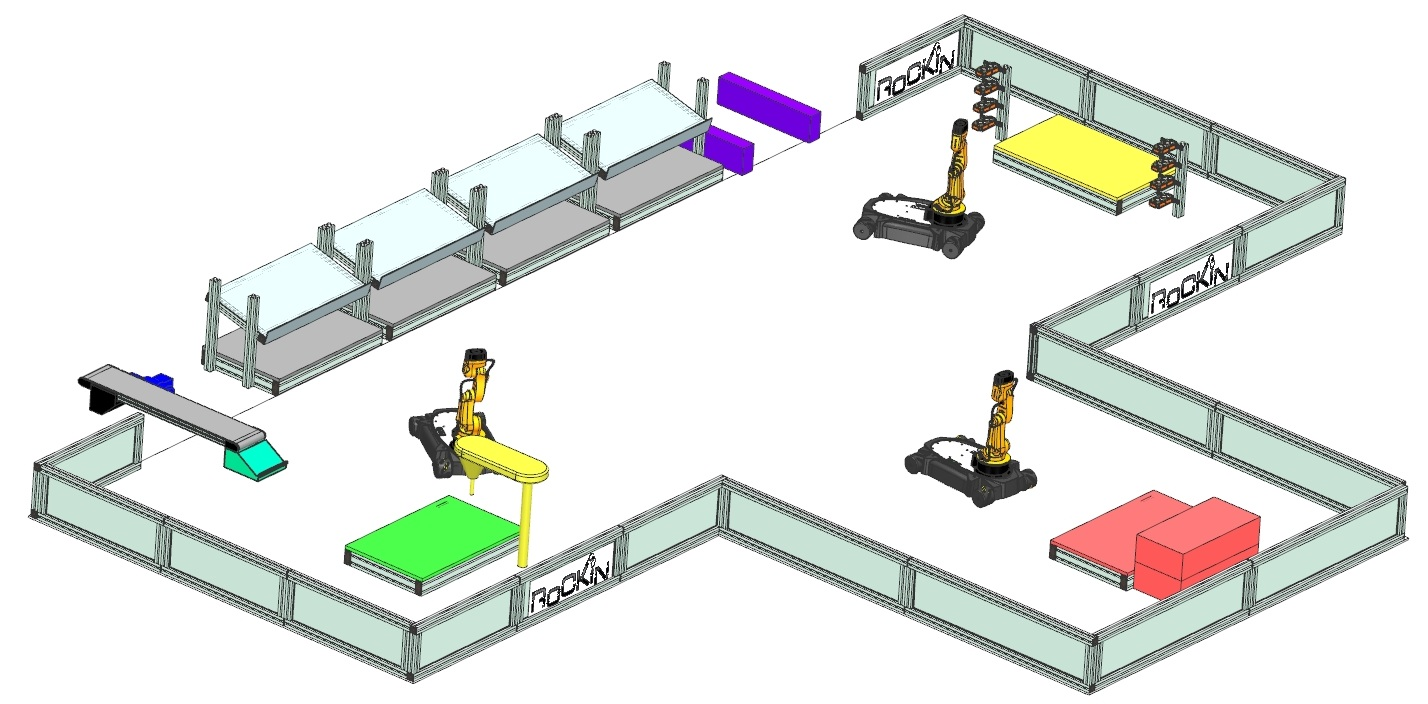
\includegraphics[height=40mm,angle=0,trim=0px 0px 0px 0px,clip]
	  		{fig/AS_RoaW_Arena_v4}
			}
		  \label{fig:NutshellArenaConcept}
		}%
		\hfill
	  \subfigure[Laboratory installation]{
		  \scalebox{1.0}[1.0]{
  		  \includegraphics[height=40mm,angle=0,trim=0px 100px 0px 200px,clip]%
	  		{pics/atwork/test_beds/WorkArenaBRSU.jpg}%
			}
		   \label{fig:NutshellArenaLab}
		}%
		\hfill
		 \subfigure[RoCKIn@Work 2014]{
		  \scalebox{.5}[.5]{%
  		  \includegraphics[height=80mm,angle=0,trim=-200px 0px -250px 0px,clip]%
	  		{pics/atwork/test_beds/WorkArena2014.jpg}%
			}%
			\label{fig:NutshellArena2014}
		}%
		\hfill
		\subfigure[RoCKIn@Work 2015]{
			\scalebox{.5}[.5]{%
				\includegraphics[height=80mm,angle=0,trim=-200px 0px -250px 0px,clip]%
				{fig/testbed/roaw_arena_lisbon.JPG}%
			}%
			\label{fig:NutshellArenaLisbon2015}
		}%
		\hfill\mbox{}
	  \caption{The evolution of the \erlir environment}
  	\label{fig:rockin-n-rollin-production-area-nutshell}
	\end{center}
\end{figure}

\noindent
An important aspect in the \erlir scenario is the development of an industry-oriented environment with ambient intelligence.
As such, the environment is equipped with various networked devices that can interact and communicate with the robot.
The following are the networked devices which are available in the \erlir environment:
%
\begin{itemize}
\item a central scheduling system (\CFH) for assigning tasks to and receiving reports from robots as well as tracking the production process and scoring of teams.
\item a quality control camera for detecting defects in the parts delivered by the conveyor belt.
\item a drilling machine.
\item a conveyor belt to deliver incoming parts from the supplier to the factory. The parts can be picked up directly on the moving belt or from the exit ramp at the end of the conveyor belt.
\item a force fitting machine.
\end{itemize}

\begin{figure}[htb]
  \begin{center}
  	\hfill
	  \subfigure[]{
		  \scalebox{1.0}[1.0]{
  		  \includegraphics[height=28mm,angle=90,trim=0px 0px 0px 0px,clip]%
	  		{pics/atwork/networked_devices/drillingMachine.jpg}%
			}
		   \label{fig:nutshellcoverPlateDrillingMachine}
		}%
		\hfill
		 \subfigure[]{
		  \scalebox{1.0}[1.0]{%
  		  \includegraphics[height=28mm,angle=90,trim=0px 0px 0px 0px,clip]%
	  		{pics/atwork/networked_devices/QCC.jpg}%
			}%
			\label{fig:nutshellcoverPlateQCC}
		}%
		\hfill
		 \subfigure[]{
		  \scalebox{1.0}[1.0]{%
  		  \includegraphics[height=28mm,angle=90,trim=0px 0px 0px 0px,clip]%
	  		{pics/atwork/networked_devices/forceFittingMachine.jpg}%
			}%
			\label{fig:nutshellForceFittingMachine}
		}%
		\hfill\mbox{}
	  \caption{Networked devices at the \erlir environment. (a) Drilling machine (b) Conveyor belt and quality control camera (c) Force fitting machine}
  	\label{fig:NutshellNetworkedDevices} 
	\end{center}
\end{figure}

%--------------------------------------------------------------------
\subsection{\erlir Benchmarks}
\label{ssec:nutshellroawtasks}


\subsubsection{Task Benchmarks}
\label{sssec:nutshellroawtasks}
The following task benchmarks can be performed:

\begin{enumerate}
	\item \textbf{\emph{Assembly Aid Tray:}} The robot's task is to collect bearing boxes from stock (shelves) and insert them into specialized aid trays. Once the assembly aid tray is filled with the bearing boxes, these aid trays are loaded to a force fitting machine, where bearings are force fitted into bearing boxes. After the bearing boxes of the assembly aid tray are force fitted, the robot needs to do a final examination before delivering the final product. By scanning identifiers (e.g. ArUco markers) as part of the task, the robot ensures tracking of the production process and the parts belonging to a particular product itself.

	\item \textbf{\emph{Plate Drilling:}} This task simulates handling incomplete or faulty parts from an external component supplier. 
	The cover plate of the bearing box has eight holes for connecting the motor with the bearing box and the four central holes need to have a cone sink. There are two possible defects of a cover plate which need to be accommodated in this task. The first case is where the supplier forgot to drill one of the cone sinks which results in a faulty cover plate. The faulty cover plates can be corrected by drilling the cone sink with the drilling machine available in the factory. The second case is where the cover plate is unusable and needs to be returned to the supplier for replacement.
	
	\item \textbf{\emph{Fill a Box (Shared with RoboCup@Work):}} The robot's task is to support a human operator in assembling a product.
	The robot must compose boxes with parts for the manual, final assembly of a drive axle. The boxes have no special subdivisions; they only can have foam material at the bottom to guarantee safe transport. Therefore, the robot has to plan the order of collecting the parts to arrange them next to each other.
\end{enumerate}

\subsubsection{Functionality Benchmarks}
\label{sssec:nutshellroawfunctionality}
The following functionality benchmarks can be performed:

\begin{enumerate}
	\item \textbf{\emph{Object Perception:}} A certain number of objects, selected from the list of \erlir items, will be positioned, one at the time, on a work area located directly in front of the robot. For each object presented to it, the robot has to perform the following activities:
	\begin{itemize}
		\item Object detection: Perception of the presence of an object on the table and association between the perceived object and one of the object classes.
		\item Object recognition: Association between the perceived object and one of the object instances belonging to the selected class.
		\item Object localization: Estimation of the 3D pose of the perceived object with respect to the surface of the table.
	\end{itemize}
	
	\item \textbf{\emph{Manipulation:}} A number of objects will be positioned, one at the time, on a table located directly in front of the robot. 
	The set of objects that will be presented to the robot is known to the robot. 
	For each object presented, the robot has to perform the following activities:
	%
	\begin{itemize}
		\item Identify which object has been presented, and provide this information.
		\item Grasp the object, lift it, and notify that grasping has occurred.
		\item Keep the grip on the object for a given time, then set the object down, release the object and move the end effector away from it.
	\end{itemize}
	Note: For this functionality benchmark, the use of any perception except vision and (if available) touch is excluded.
	
	\item \textbf{\emph{Control:}} This functionality benchmark assesses the robot's capability of controlling the manipulator (and the mobile platform) motion in a continuous manner. 
	This functionality is essential for precise placement of objects or following a given line in common industrial applications (e.g. welding).
	A marker set is attached to the robot's manipulator. With the tip of this marker set, the robot has to follow a given path in Cartesian space. The external ground truth system measures the deviation between the given path and the path executed by the robot using this marker. Only for visualization purposes, the path is displayed on the table
	
	\item \textbf{\emph{Navigation (Shared with RoboCup@Work):}} This functionality benchmark assesses the robot's navigation capability. 
	This functionality is essential for efficient delivery of objects.
	In this benchmark the robot receives an ordered list of waypoints that it must reach. The robot must follow the order and send back a signal each time it reaches a waypoint. The evaluation of the navigation will take into account the distance between the robot's position and the respective position of the waypoint, the difference in the orientation and the time spent by the robot to go from each waypoint to the next waypoint.
	\end{enumerate}

%--------------------------------------------------------------------
\subsection{Robots in the \erlir competition}
The \erlir competition is designed for robot platforms with mobile manipulation capabilities such as presented in Figure \ref{fig:roawRobots}.
Additionally, it is possible to compete with a new robot prototype. 
For example a robot platform built from the integration of a mobile base with a manipulator (e.g. ABB IRB 120, Neuronics Katana, Robotis Manipulator-L, Robai Cyton Gamma 1500, Barrett WAM, Universal Robots UR5). 
Obviously, the robot used for the competition should consider the competition arena which is a scaled down version of the typical small- to medium-sized factory production area.

\begin{figure}[htb]
	\begin{center}
		\hfill
		\subfigure[Robotnik X-WAM \newline \href{http://www.robotnik.eu/manipulators/x-wam/}{www.robotnik.eu}]{
			\scalebox{1.0}[1.0]{
				\includegraphics[height=34mm,angle=0,trim=40px -40px 40px -40px,clip]%
				{fig/roawRobots/robotnik-x-wam.jpg}%
			}
			\label{fig:XWAM}
		}%
		\hfill
		\subfigure[Neobotix MM-500 \newline \href{http://www.neobotix-robots.com/mobile-manipulator-mm-500.html}{www.neobotix-robots.com}]{
			\scalebox{1.0}[1.0]{
				\includegraphics[height=34mm,angle=0,trim=-10px -5px -10px -5px,clip]%
				{fig/roawRobots/MM-500Neobotix.jpg}%
			}
			\label{fig:MM500}
		}%
		\hfill
		\subfigure[KUKA youBot]{
			\scalebox{1.0}[1.0]{
				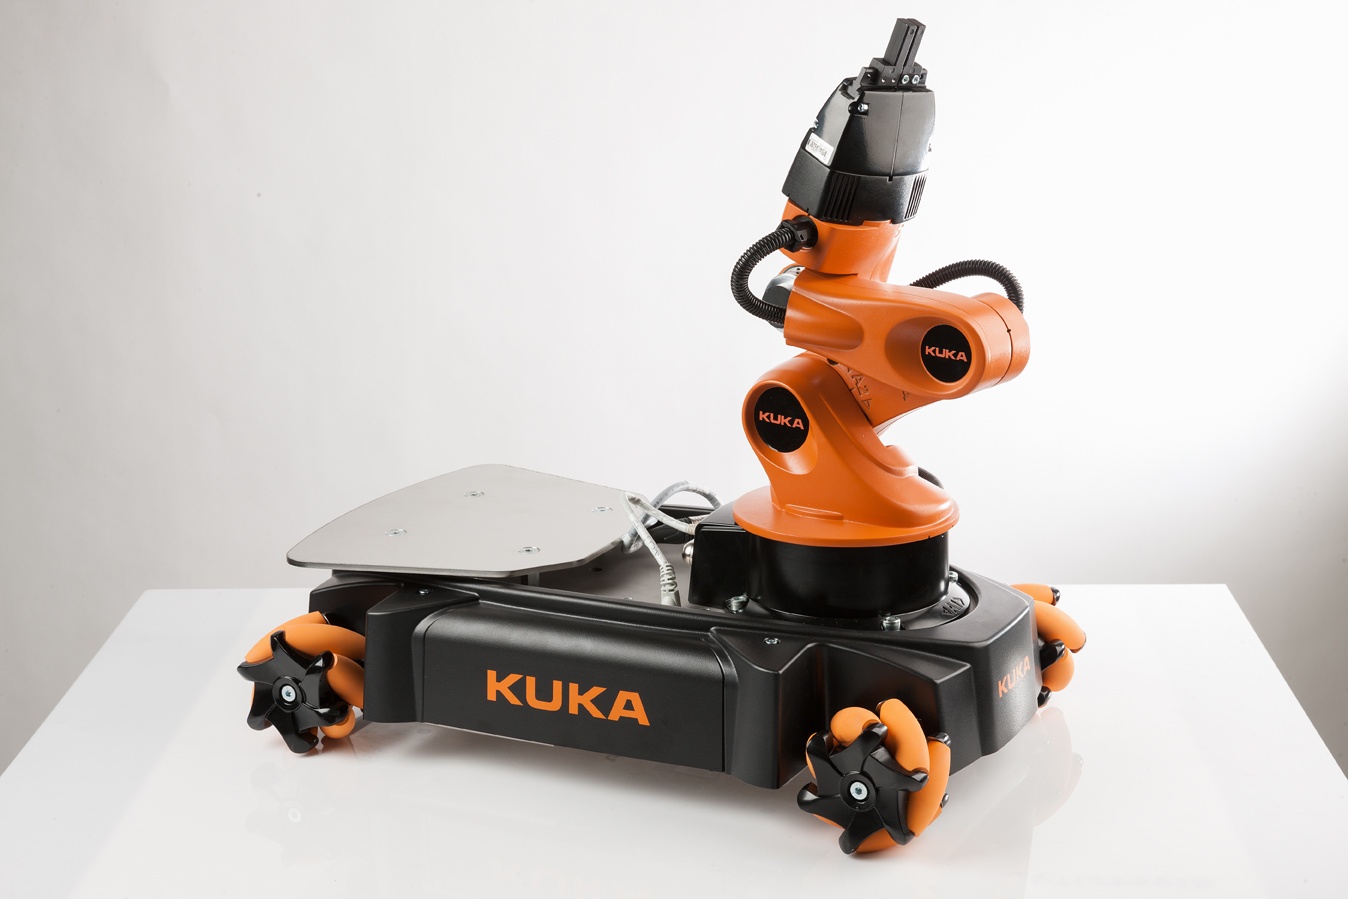
\includegraphics[height=34mm,angle=0,trim=40px 0px 40px 0px,clip]
				{fig/robots/youbot/youBotFinal.jpg}
			}
			\label{fig:youBot}
		}%
		\hfill\mbox{}
		\caption{Example of mobile manipulators for \roaw}
		\label{fig:roawRobots} 
	\end{center}
\end{figure}

The robot must be operated in fully autonomous mode when completing each task, i.e. neither power supply via cable nor any kind of teleoperation is permitted.
Networked devices will be prepared by the organizer to interact and cooperate with the robot during the execution of the \erlir tasks.
